%%% Partnership for Advanced Computing in Europe 
%%%   www.prace-ri.eu
%%%
%%% LaTeX template for a PRACE-RI whitepaper.
%%%
%%% (c) CSC - IT Center for Science Ltd.
%%%   author: Martti Louhivuori (martti.louhivuori@csc.fi)
%%%
%%% Generic instructions:
%%%   - follow the point-by-point instructions
%%%   - fill in the required author information, title, and abstract
%%%   - write your paper using the general format outlined below
%%%   - do NOT touch the generic layout between the following tags: 
%%%       %%% PRACE GENERIC LAYOUT; DO NOT CHANGE %%%
%%%       %%% END OF PRACE GENERIC LAYOUT %%%
%%%   - the paper should be 3-6 pages long
%%%   - refer to 'example.tex' and 'example.pdf' for a practical example
%%%
%%% PRACE GENERIC LAYOUT; DO NOT CHANGE %%%
\documentclass{prace}
%%% END OF PRACE GENERIC LAYOUT %%%

% TITLE
%   - use the name of your project
%   - capitalise the first letter
\title{}

% AUTHORS
%   - include all people involved in the effort
%     - depending on their contribution, include PRACE experts as authors 
%       or mention them in acknowledgements
%   - give affiliations in the option field as a list of numbers 
%     corresponding to the order of \affiliation definitions, i.e. 
%     [1] -> 1st \affiliation, [2] -> 2nd, [1,2] -> 1st & 2nd
%   - mark one of the authors as the corresponding author using
%     \corresponding before the \author, i.e. 
%       \corresponding\author[1]{N.N.}
%
% example:
%   \author[1]{First Author}
%   \corresponding\author[2]{Second Author}
%   \author[1,2]{Third Author}
\author[]{}
\corresponding\author[]{}

% AFFILIATIONS
%   - define affiliations in the same order you used for in the author 
%     definitions
%   - include: name, address, city, postcode, and country
%
% example:
%   \affiliation{First affiliation, Address, City and Postcode, Country}
%   \affiliation{Second affiliation, Address, City and Postcode, Country}
\affiliation{}

% PROJECT ID
%   - use the ID of your project
\project{}

% CONTACT INFORMATION
%   - give the email address of the corresponding author
%
% example:
%   \email{second.author@example.com}
\email{}

%%% PRACE GENERIC LAYOUT; DO NOT CHANGE %%%
\begin{document}
\maketitle
%%% END OF PRACE GENERIC LAYOUT %%%

% ABSTRACT
%   - write a concise abstract that outlines the approach / methods, main 
%     results, and relevance of your project
\begin{abstract}
\end{abstract}

% MAIN BODY
%
% Write the report in the style of a journal article (i.e. Introduction, 
% Methods, Results, Conclusions). The appropriate length of the paper 
% is 3-6 pages (although there is no upper limit).
%
% In the report please describe:
%   - goals of the project
%     - scientific case and goals related to the project
%     - technical goals (performance, parallel scalability, ...)
%   - work done in the project, including
%     - technical and algorithmic methods and programming techniques employed
%     - use of profiling tools when applicable
%     - use of  numerical libraries when applicable
%     - machine(s) used for the work
%   - results obtained
%     - give quantitative measurements of the achieved performance 
%       enhancements and the scaling behaviour
%     - discuss how the results compare with the goals
%   - summary
%     - relevance of the obtained results for the stated scientific goals
%     - outlook on possible future work
%
% instructions:
%   - use only \sections and \subsections to divide the paper into logical 
%     segments
%   - capitalise only the first letter of headings
%   - symbols denoting vectors and matrices should be in bold type
%   - scalar variables should be in italics, i.e. enclosed within $$ in text
%   - weights and measures should be expressed in SI units
%   - avoid footnotes if at all possible
%   - collate acknowledgements in a separate section at the end of the 
%     article; do NOT include them on the title page, as a footnote etc.
%
% example:
%   \section{Introduction}
%     Introductory text...
%   \section{Methods}
%     General description...
%   \subsection{Specific method A}
%     Method A in detail...
%   ...
%   \section{Acknowledgements}
%     The results in this paper have been achieved using the PRACE Research
%     Infrastructure. 
%     
\section{}
\subsection{}

% FIGURES
%   - all photographs, schemas, graphs, and diagrams are to be referred to 
%     as figures
%   - line drawings should be goo quality scans or true electronic ouput
%   - low-quality scans are not acceptable
%   - lettering and symbols should be clearly defined either in the caption 
%     or in a legend provided as part of the figure
%   - figures should be placed at the top or the bottom of a page whenever
%     possible
%   - if two images fit next to each other, they may be placed so to save
%     space
%   - refer to figures in the text as Fig.~\ref{fig: foo} (with the correct 
%     reference labels of course)
%
% examples:
%   - single image:
%     \begin{figure}
%       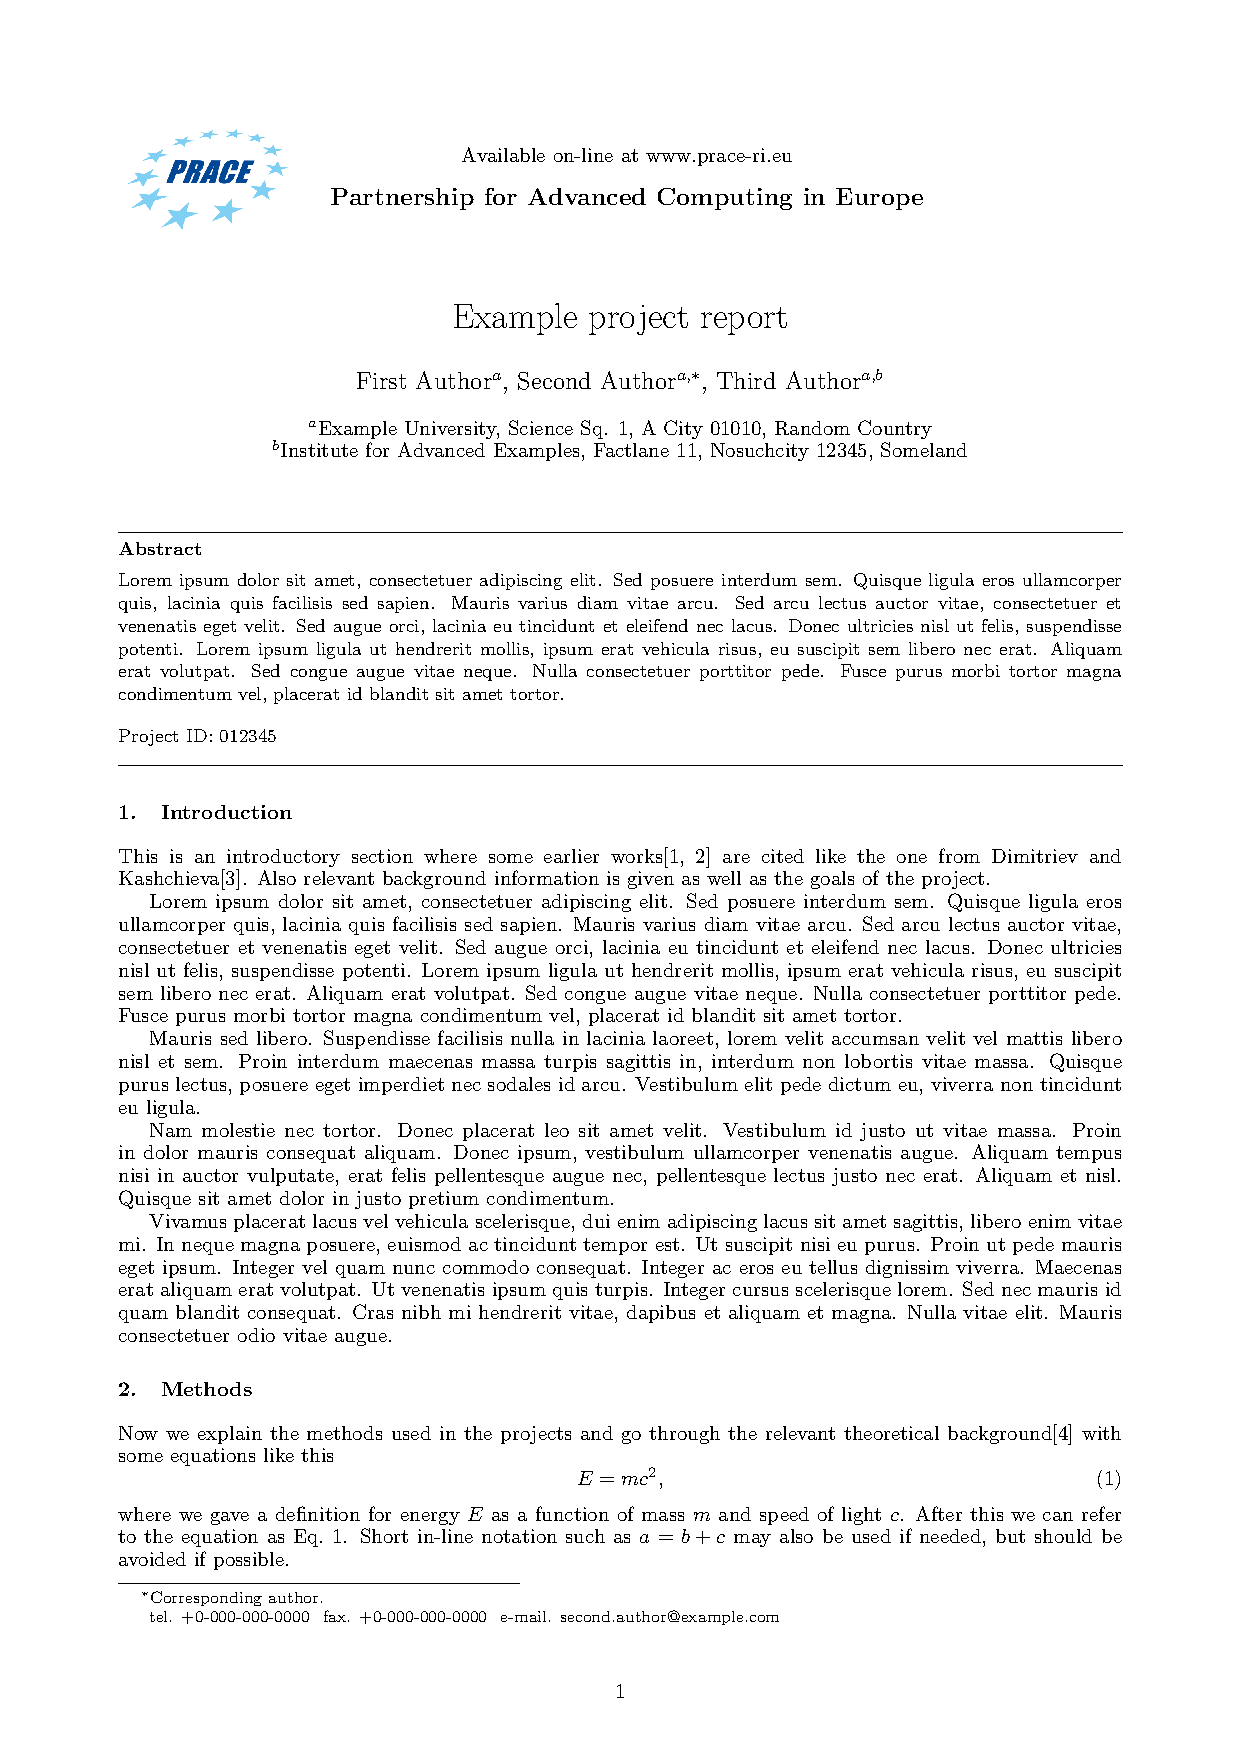
\includegraphics[width=0.4\textwidth]{example}\hfill{}
%       \caption{singlepicture}
%       \label{fig: single-example}
%     \end{figure}
%
%   - two images side-by-side:
%     \begin{figure}
%       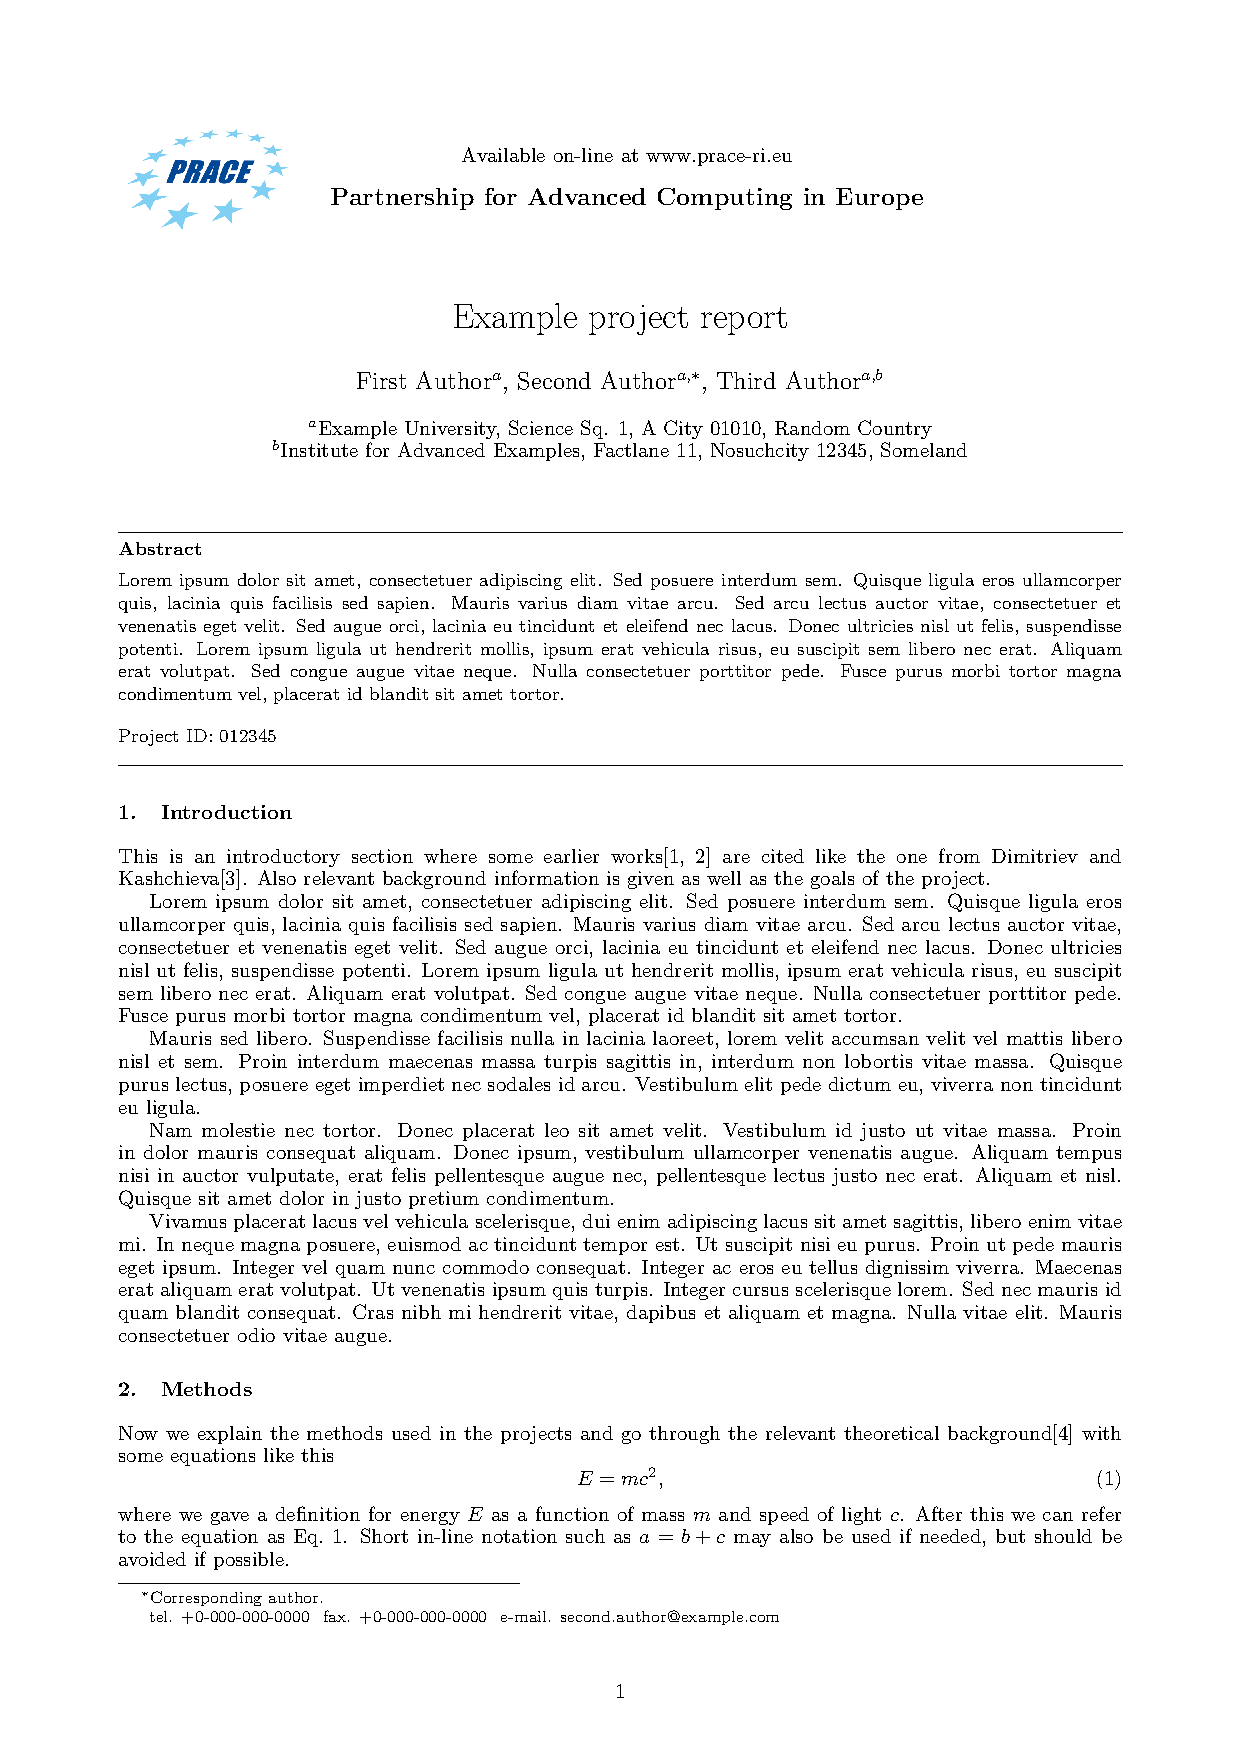
\includegraphics[width=0.4\textwidth]{example}\hfill{}
%       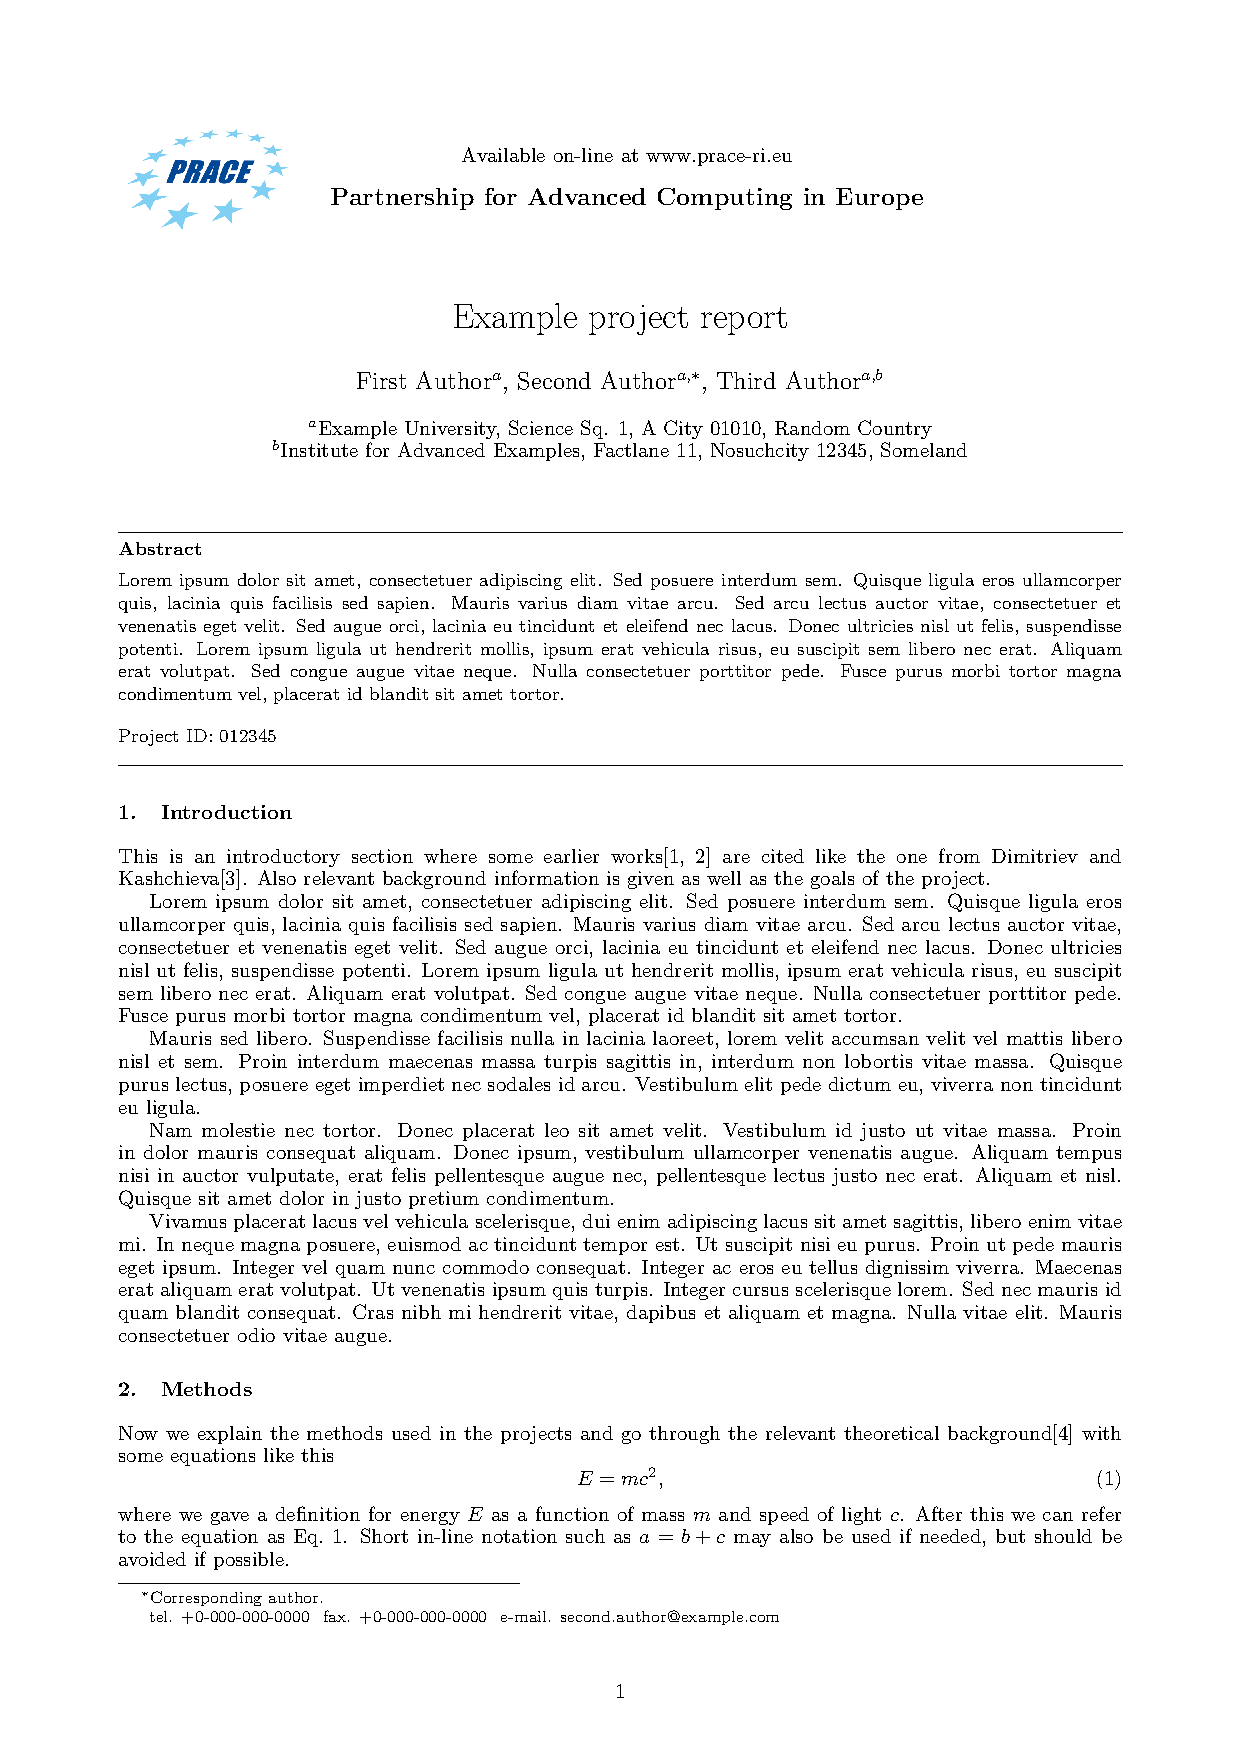
\includegraphics[width=0.4\textwidth]{example}\hfill{}
%       \caption{(a) first picture; (b) second picture}
%       \label{fig: double-example}
%     \end{figure}
\begin{figure}
	\includegraphics[]{}\hfill{}
	\caption{}
	\label{}
\end{figure}

% TABLES
%   - tables must be embedded into the text and not supplied separately
%   - caption before tabular
%   - left-justified columns
%   - only horisontal lines within a table:
%       - \toprule at the beginning of the table
%       - \midrule after the column headings but before the body
%       - \bottomrule at the end of the table
%   - \cmidrule can also be used for partial lines within the column headings 
%     (see the booktabs package documentation for further details: 
%      http://www.ctan.org/tex-archive/macros/latex/contrib/booktabs/ )
%   - refer to tables in the text as Table~\ref{tab: foo} (with the correct 
%     reference labels of course)
%
% example:
%   \begin{table}
%     \caption{An example of a table}
%     \label{tab: example}
%     \begin{tabular}{lll}
%       \toprule 
%       An example of a column heading & Column A (t) & Column B (T) \\
%       \midrule
%       An entry & 1 & 2 \\
%       and another entry & 3 & 4 \\
%       yet another entry & 5 & 6 \\
%       \bottomrule 
%     \end{tabular}
%   \end{table}
\begin{table}
	\caption{}
	\label{}
	\begin{tabular}{}
		\toprule
		\midrule
		\bottomrule
	\end{tabular}
\end{table}

% LISTS
%   - use \itemize for bulleted lists and \enumerate for numbered lists
%
% example:
%   \begin{itemize}
%     \item First point
%     \item Second point
%   \end{itemize}
\begin{itemize}
	\item 
\end{itemize}

% REFERENCES
%   - use \cite for references
%   - always include \cite even when referring to the authors by name
%
% example:
%   Example citation to a paper\cite{scholes-DiscussFaradaySoc-70} and to 
%   another paper by Someone \emph{et al.}\cite{someone-SomeJournal-00}.
\cite{}

% EQUATIONS
%   - use the equation environment for all equations
%   - short in-line notation may also be used, but should be avoided if
%     possible
%   - use bold type face (\mathbf) for vectors and matrices
%   - refer to equations in the text as Eq.~\ref{eq: foo} (with the correct 
%     reference labels of course)
%
% example:
%   \begin{equation}
%     Rt = K EP = 93.02 (\pm 9.62) – 13.45
%     \label{eq: example}
%   \end{equation}
\begin{equation}
	\label{}
\end{equation}

% ACKNOWLEDGEMENTS
%   - additional acknowledgements may be added
%   - names of PRACE machines and the corresponding sites and countries
%     should be inserted to end of the general PRACE acknowledgement 
\section*{Acknowledgements}
This work was financially supported by the PRACE project funded in part
by the EUs 7th Framework Programme (FP7/2007-2013) under grant agreement
no. RI-211528 and FP7-261557. The work is achieved using the PRACE 
Research Infrastructure resources [insert here machine names and the 
corresponding sites and countries].

% REFERENCE LIST
%   - use \thebibliography and \bibitems to enter references, no separate .bib
%     files
%   - use normal font for *everything* (no bold typefaces etc.)
%   - shorten the last page number, i.e. 51--9 for pages 51--59
%   - for more than 6 authors the first 6 should be listed followed by et al.
%     - use \emph{et al.} for the et al.
%   - end each reference with a period
%
% example:
%   \begin{thebibliography}{99}
%     \bibitem{scholes-DiscussFaradaySoc-70}
%       S. Scholes, Discuss. Faraday Soc. No. 50 (1970) 222.
%     \bibitem{mazurin-Phase-Separation-in-Glass-84}
%       O.V. Mazurin and E.A. Porai-Koshits (eds.), 
%       Phase Separation in Glass, North-Holland, Amsterdam, 1984.
%     \bibitem{dimitriev-JMaterSci-75}
%       Y. Dimitriev and E. Kashchieva, J.Mater. Sci. 10 (1975) 1419.
%     \bibitem{eaton-Porous-Glass-Support-Material-75}
%       D.L. Eaton, Porous Glass Support Material, US Patent No. 3 904 422 
%       (1975).
%   \end{thebibliography}
\begin{thebibliography}{99}
	\bibitem{}
\end{thebibliography}

%%% PRACE GENERIC LAYOUT; DO NOT CHANGE %%%
\end{document}
%%% END OF PRACE GENERIC LAYOUT %%%
